\chapter{Implementation: DApp}
DApp is often described as P2P, trustless with a special characteristic that there is not a single server to control it. DApp includes at least one User interface or frontend that could be a Mobile app, Desktop application installed on a computer.\\
The data relating to the application could be provided by a single group or company or may provide by end users themselves. Finally, it involved some kind of data manipulation. \\
DApp uses the ethereum as backend of its data storage and processing using smart contracts. The user interface of DApp is usually like traditional websites but is one website plus one or multiple smart contracts.

\begin{center}
	
	\begin{figure}[htb!]
		
		\begin{minipage}{0.75\linewidth}
			
			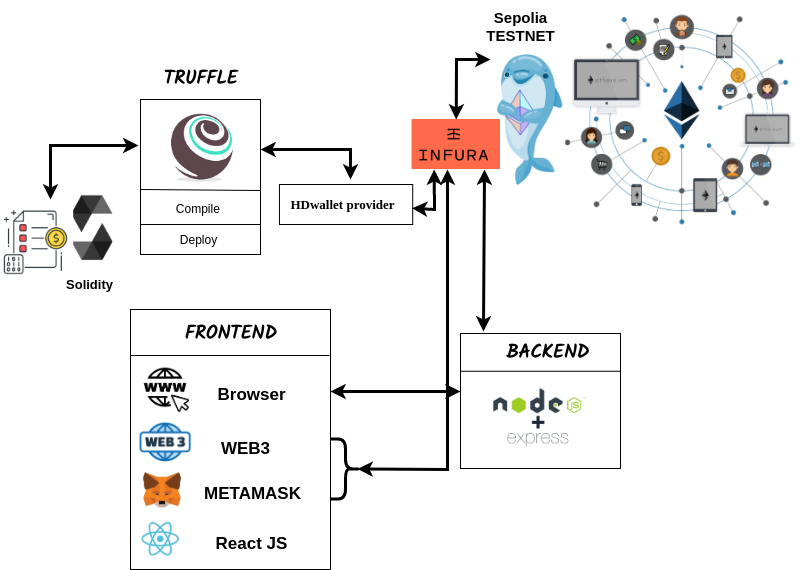
\includegraphics[width=1.45\textwidth]{images/chap03_dapp.png}
		\end{minipage}
		\caption{DApp infrastructure}
		
	\end{figure}
	
\end{center}

\section{DApp and Ethereum Blockchain}
The benefit of using the Ethereum blockchain in DApps are as follows:
 \begin{itemize}
     \item 1- The user can see what is going on before submitting any data.
     \item 2- Once the user has interaction, no one can temper or delete data.
     \item 3- The user of the application can directly participate in application management.
 \end{itemize}
\section{Project Concepts}

In this section, we focused on the requirements that we need to address in our application.
\\
\subsection{Contract and Ontology Specification}
Here, it is explained some terms related to smart contracts and the ontology of our application. And we needed them as the primary requirement to build up this dApp.
\begin{itemize}
	\item \textbf{Definition 1 (Owner)} is the address of deployed contract or transaction to the blockchain. That is the first person who interacts with the contract. In this case, the owner can change her/his license of the file.\\
	\item \textbf{Definition 2 (Non-owner)} is the another user that make not action. In this case, can retrieve license information related to specific files.\\
	\item \textbf{Definition 3 (Licensor)} is the address currently interact with smart contract. In this case, can license his/her file.\\ 
	\item \textbf{Definition 4 (Semantic mappings)}: As we do not have the authority to change stored data on the Ethereum blockchain, one idea is to create a template to have a semantic view of the blockchain.
	To reach this purpose, we need a mapping between stored transaction data in the blockchain and transaction concepts defined as ontology, then make a query on produced data from this mapping. This process consists of three following requirements:
	
	\begin{itemize}
		\item \textit{Transaction Schema} are actually some attributes resulted from web3.eth functions that EhtOn data properties would be mapped to.
		\item \textit{Transaction Triple template} defines for the relationship between concepts(block or transaction) and properties. It is known as 'Subject predicts Object' that Subject is the web3.eth properties, predict known as EthOn ontology predictor(data properties) and Object (web3.eth properties) is a place that would be replaced by the transaction schema on the mapping. 
		\item \textit{Triplize} is the function that generates data in RDF format by creating a mapping between the two above parameters as input. 
	\end{itemize} 
     \item \textbf{Definition 5 (Prefix)} name is the label or local part separated with ':' and is the abbreviation of terms that referenced resources explicitly. According to Wikipedia, Prefixes are declared on the top of the SPARQL query and our triple template, so that the statements can reference to.\\
     \textbf{Definition 6 (Triple)} defined in Wikipedia as a statement with three entities that codifies semantic data in the form of \textit{Subject-predict-Object} expressions.\\
\end{itemize}
\subsection{Technology Usage}
\textbf{DApp} \\
It is a type of open-source smart contract application that runs on a decentralized peer-to-peer network rather than a centralized server. It allows users to transparently execute a transaction on a distributed network. \\
DApp is similar to centralized apps, as they use frontend and backend. But the backend's app is supported by a centralized server or database. And Backend's DApp runs on a decentralized p2p network and is supported by smart contracts which store on the Ethereum blockchain.\\
\\
\textbf{Decentralized application characteristic:}\\
	\textit{Open Source}: all the required are decided on a census of all available users on a network.\\
	\textit{Decentralized Storage}: data is stored on decentralized blocks.\\
	\textit{Validation}: As the application runs on blockchain. They offer validation of data using cryptographic tokens which are needed for the network. \\
 \\
\textbf{Ethereum} \\
it is explained in section 1.4.\\
\\
\textbf{Solidity} \\
it is explained in section 1.5.5.\\
\\
\textbf{SHA3-256} \\It is explained in section 1.5.3.
\textit{message} is the additional input parameter in text type\cite{fips}.\\
\textbf{Java Script Tools} 
\begin{itemize}
  \item \texttt{Truffle} is the smart contract development tools and testing network for blockchain applications and supports developers who are looking to build their dApp, etc. \\
 Truffle offers some different features: \\
 \textit{- Smart contract Managing}: truffle helps to Manage artifacts of smart contracts used in dApp and supports library linking, deploying, and some other Ethereum dApps. \\
 \hspace{3cm} \textit{- Contract testing system}: Truffle helps developers construct smart contract testing systems for all their contracts. \\
 \textit{- Network management} helps developers by managing their artifacts. \\
 \textit{- Truffle console} allows the developer to access all truffle commands and built contracts \footnote{https://moralis.io/truffle-explained-what-is-the-truffle-suite}.
\\
\item \texttt{React. js} is an open-source JavaScript framework which used as a frontend. In react, a developer builds a web application by using reusable individual components that are assembled from an application's whole user interface.\\
React has the advantage of providing a feature that combines the speed of JavaScript with a more efficient method of managing DOM to render web pages faster and create more responsive web application \footnote{https://blog.hubspot.com/website/react-js}.\\
\item \texttt{crypto. js} is the JavaScript library that performs data encryption and decryption. It is a collection of standard algorithms including SHA3-256 \footnote{{https://github.com/jakubzapletal/crypto-js}}.
\item \texttt{Web3.js} helps developer to connect to Ethereum blockchain. It is a collection of libraries that allows developers to perform some actions like sending ether, checking data from smart contracts, and creating smart contracts \footnote{https://www.datastax.com/guides/what-is-web3.js}.\\
\item \texttt{axios} provides the HTTP requests from the browser and handles request/response data \footnote{https://axios-http.com/docs/intro}. \\
\item \texttt{HDwallet provider} is a package to help the developer to connect to the network. It is easy to configure the connection network to the Ethereum blockchain through \textit{infura}. This provider is used by Truffle when we deploy the contract. In addition, meta mask providers are also used when we want to interact with the contract in the browser.\\
HDwallet provider provides a custom URL: 'http://127.0.0.1:7545'. This will spawn a development blockchain locally on port 7545 \footnote{https://github.com/trufflesuite/truffle-hdwallet-provider}. \\
\item \texttt{Express.js} is node.js framework for authority dApp. It provides HTTP methods (GET, POST) to call functions for particular URL routes \footnote{https://www.simplilearn.com/tutorials/nodejs-tutorial/what-is-express-js}. \\ 
When we run dApp, we have an HTTP server located on port 3000. \\
\item \texttt{FS} provides some functionality to interact with the file system, mostly used functions like: \textit{readFileSync}, \textit{writeFileSync} and \textit{appendFileSync} \footnote{https://blog.risingstack.com/fs-module-in-node-js/}. \\
\end{itemize}

\textbf{Semantic Web Tools}\\
\begin{itemize}
	\item \textit{EthOn Ontology} is semantic view of ethereum blockchain. It encompasses different classes and relations to cover different concepts of Ethereum like blocks, transactions, and messages to formalize RDF triple. We used classes and properties related to transaction concepts as a template to model our transaction to DALICC \footnote{https://axios-http.com/docs/intro}.
	\item \textit{SPARQL query} is defined in the section 2.1.4.
	\item \textit{Command-Line SPARQL with Jena} is a utility of Apache Jena that runs queries on remote SPARQL endpoint or RDF files that would be lo located on a local computer or web. We used the command as follows:\\
	 - Using Command line : \textit{sparql --data rdfFile --query sparqlFile}
	
\end{itemize}
\textbf{Ethereum Tools}

\begin{itemize}
\item \textit{Infura}, According to the internet definition, a web3 backend and infrastructure-as-a-Service (IaaS) provider offers a range of tools to help the developer to build dApp to connect to the Ethereum blockchain.\\
\item \textit{Metamask Wallet} Metamask is a wallet used to interact with the Ethereum blockchain. It allows users to connect network through a browser extension or mobile app. Metamask wallet, including all accounts, each account has its private key \footnote{https://originstamp.com/blog/metamask-what-is-it-and-how-does-it-work/}.\\
\item \textit{Faucet(ETH faucet)} is the platform that gives some test tokens to a user to test smart contracts or send transactions before deploying them to the main net. \\
\item \textit{Testnets} are the test blockchain networks that perform similarly to the main blockchain (mainnet). This allows developers to execute their contracts on test blockchain freely \footnote{https://blog.infura.io/post/introducing-infuras-eth-testnet-faucet-get-0-5-eth-daily-to-test-your-dapps}.\\
Infura's new testnet faucet is Sepolia ETH which provides the most reliable and high-volume faucets for developers. \\
\item \textit{Web3.eth} the package that allows interacting with the Ethereum blockchain. It contains many functions to provide more information about executed smart contracts or transactions on the blockchain. 
In our case, some functions including: \textit{getBlock}, \textit{getTransaction} and \textit{getTransactionReceipt} are used to provide some more details which are mapped to Ethan ontology objects properties. These retrieved properties would be used later in triple.\\
\item \textit{- knowledge graph} provided to indicate classes and relations.
The idea is to use a graph-based data model to clarify survived transaction, their classes, and relations in much more detail. 
\begin{center}
	
	\begin{figure}[htb!]
		
		\begin{minipage}{0.75\linewidth}
			
			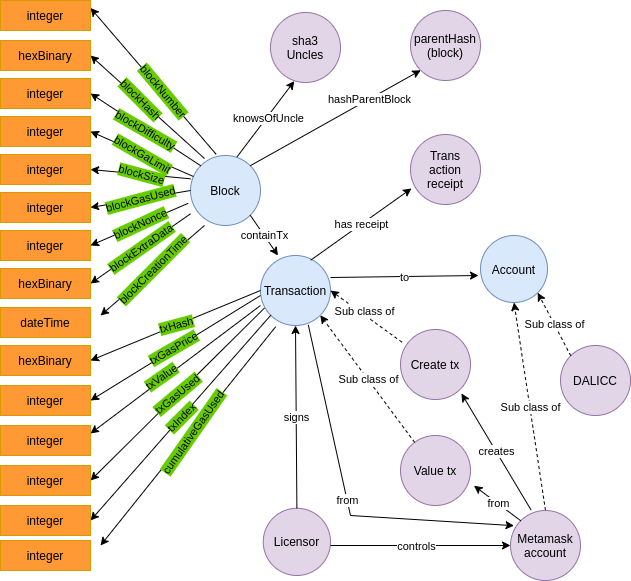
\includegraphics[width=1.45\textwidth]{images/chap03_knowledge_graph.png}
		\end{minipage}
		\caption{Transaction illustration}
		
	\end{figure}
	
\end{center}

\end{itemize}
\section{Project Architecture}

\subsection{Backend} The backend of this project relies on the Ethereum platform using smart contracts. In addition, DALICC license library the user can license here/his data or retrieve license information. In the next paragraph, we will more focused on authenticated users as the main challenge in decentralized apps and data licensing systems by users. \\
\\
\textbf{Authenticated user} \\
Authentication of users on Ethereum for validation purposes is the essential feature when building dApp.  Therefore, programming the functionality of Ethereum authentication for dApps is important for blockchain developers. 
In this dApp, we consider two solutions for Ethereum authentications as follows: \\
\\
\textit{- login to metamask:} Metamask is the most popular cryptocurrency wallet (Ethereum account) to support the Ethereum blockchain. Additionally, metamask is a bridge for web3 authentication to an Ethereum-based decentralized application. By logging into Metamsk, users can submit transactions or check the stored data on the blockchain.\\
\textit{- Using smart contract: } The address of the metamask is passed to smart contract as a licensor, then it will
use this address as an owner to license his/her file. \\
\\
\textbf{Licensing in smart contract} as follow: \\
\\
\textbf{License information} represents three elements: licensor address that is passed by metamask, license of data, and the URI related to this license.\\
\textbf{Storage license information}: Each smart contract that runs on the Ethereum blockchain would be maintained state in its permanent storage. The license information is stored in its storage and is changeable only by the smart contract itself.\\
\textbf{Retrieve license information}\\
As mentioned earlier, only a smart contract can change the data in its memory. Thus, we can consider smart contracts a validating system for license requests. The JavaScript
library web3.js is an interface to the Ethereum Network for the frontend of this dApp. This allows the frontend to access the smart contract, retrieving or changing license information.\\

\subsection{Frontend}
 Frontend of this project build on React.js, HTML, and CSS. The React js used in this front-end for the user interface.\\
 \\
 \textbf{User roadmap}\\
 The licensing Data from the user interface includes three phases:
 \begin{itemize}
 	\item The user gets asked to select to license type from which to be loaded from Dalicc Library via Axios and get a request in frontend. Then, after selecting data in the next field, the user should check the file, if the selected file is already licensed or not. Depending on this verification, the user receives either the confirmation message 'License detected' or the rejection message 'License not detected'. 
 	\item The user should go further by pressing the 'License Data/ retrieve license' button to get license information for the confirmation message of the last phase or license his/her file.\\
 License information contains some information like license type, license URI retrieved from the DALICC library, and the address of the owner of this license. For licensing data, the user gets asked to log in to Metamask for the authentication process and this address would be passed to smart contract as owner of this license. The licensing process will be done by receiving the hash value of licensed data.
 	\item In the last phase, the user can observe receipt of this transaction in a table that contains transaction details from the interaction between \textit{web3.eth} and \textit{ethOn ontology}.
 \end{itemize}
 \begin{center}
 	
 	\begin{figure}[htb!]
 		
 		\begin{minipage}{0.75\linewidth}
 			
 			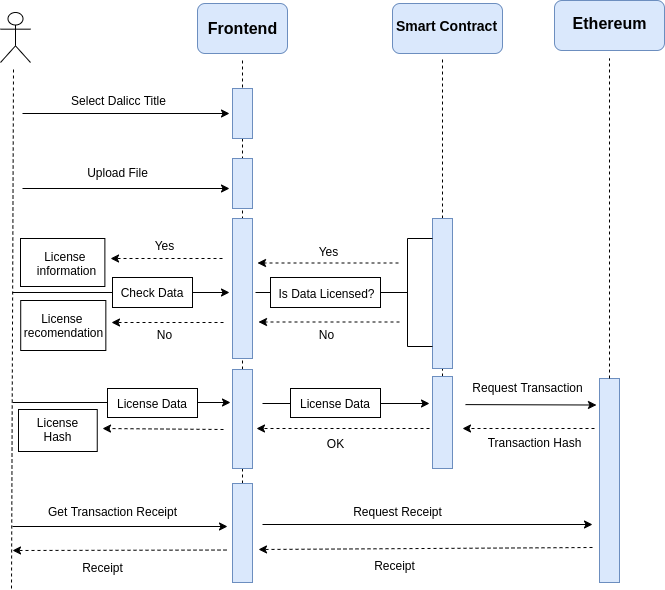
\includegraphics[width=1.45\textwidth]{images/chap03_user_roadmap.png}
 		\end{minipage}
 		\caption{Sequence diagram for licensing file}
  	\end{figure}
  \end{center}
 \textbf{Interaction with backend}\\
 Since the backend code(smart contract) of the dApp is on a decentralized network, we focused on the interaction between the smart contract and the Ethereum network. The communication between the fronted and backend is taken over by Java Script library \textit{web3.js}.
 For this purpose, web3 provides this connection either with HDWallet-provider to connect to the test network (Sepolia in our case) or Ethereum provider.\\
 \\
 \textbf{Interaction with with DALICC} \\
 To retrieve the license, an HTTP GET request is sent to the DALICC library endpoint and returns the license which encompasses two elements: license title and license URI. The user can choose just the DALICC title as a license then the URI of the associated title would be stored subsequently in the smart contract for further processing. \\
 \\
\textbf{License receipts}\\
After committing a transaction in the blockchain, the user can get transaction details via web.eth, then send transaction details in RDF format to the server to store into a file. The produced turtle file will be resulted into a readable format and would be returned to frontend by HTTP GET request from frontend.
\\
\subsection{DApp Architecture} 
This application encompasses some components:
\begin{itemize}
	\item User interface
	\item Smart contract to communicate with DALICC library
	\item Ethereum network to support transaction
	\item Transaction receipt
	\item EthOn ontology
	\item SPARQL query    
\end{itemize} 
\begin{center}
   \begin{figure}[htb!]
		
		\begin{minipage}{0.75\linewidth}
			
			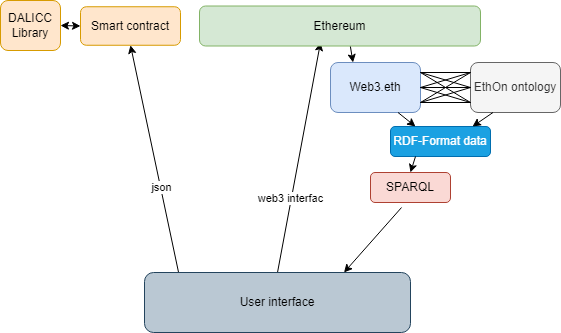
\includegraphics[width=1.5\textwidth]{images/chap03_eth_dalicc_comm.png}
		\end{minipage}
		\caption{DApp Architecture}
	\end{figure}
\end{center}

\section{Implementation}
This section comprises the implementation details in a smart contract and some main functions in the application.

\subsection{Smart Contract Logic}
As mentioned before, the backend code of this application is on the Ethereum network. in this section, we will contemplate more on each functionality of the contract in this dApp.
\begin{itemize}
	\item \textit{Owned contract} \\
	This smart contract contains the function to prevent non-owner users to call the function and the owner as the constructor to be usable in every contract which is called to. This contract provides a function that helps us to restrict access to some function in another contract that would be called later by them. \\
	\item \textit{PrimaryLicenseContract} \\
	This is the main contract that communicates with two other contracts to represent the public interface of the licensing system. It provides functions to licensing data or retrieves license information. \\
   \item \textit{LicenseManager contract} \\
	This smart contract is responsible for saving the address of the license or creating one for the new file. \\
	\item \textit{License contract} \\
	In this contract, the hash value and licensor address would be stored here. License contracts represent only one license and associate license contract for this license. The license contract should have been created by the license manager.

\end{itemize}

\begin{center}
	
	\begin{figure}[htb!]
		
		\begin{minipage}{0.75\linewidth}
			
			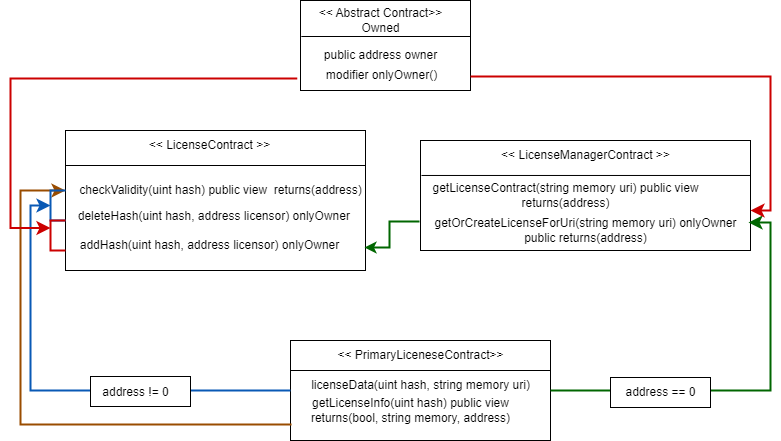
\includegraphics[width=1.45\textwidth]{images/chap03_smartContract_visual.png}
		\end{minipage}
		\caption{Smart contract visualization}
		
	\end{figure}
	
\end{center}

\text{How Smart Contract works?}

\begin{itemize}
	\item \textbf{Licensing system process} \\
	To license data, two parameters are needed. The first one is the hash of related data and the second one is the address related to the URI of the license. This smart contract as a \textit{caller} take over the process: \\
	\textbf{License data} \\
	To license data, the function \textit{licenseData} is used which declares with two parameters: the first one is the hash associated with selected data, and the second one is the URI of the selected license. By pressing the 'License Data/retrieve license on the frontend, the function
	\textit{licenseData} would be triggered and perform the steps as follow: \\
	This function checks if the target address is the zero account, which means the transaction creates a new contract: 
	if no, function \textit{deleteHash}, otherwise \textit{getOrCreateLicenseForUri} would be called. How does licensing data work? \\
	\begin{itemize}
		\item \textit{licenseData} function check if the specified hash is linked to a license and the caller is licensor, then \textit{deleteHash} is called and the hash of related data and address of licensor would be passed. \\
		\hspace{1cm} \textbf{Definition} \textit{deleteHash}: This function is accessible just for the owner (function caller), which means the caller of this function must be the owner and the passed address should be the licensor. Then the link between the hash and license will be dropped.
		\item \textit{getOrCreateLicenseForUri} of the license Manager is called and the URI of the selected data as input parameter would be passed and returns the address to license contract which represents this URI.\\
		\hspace{1cm} \textbf{Definition} \textit{getOrCreateLicenseForUri}: This function checks if the caller of this function is the owner, then exists a license contract for a given URI. If so, the address of this license contract would be returned. Otherwise, a new license contract will be created and the address of the contract will be stored and returned. The caller's address of the caller also will be used later as the owner of this contract.
		\item \textit{addHash} function of the License contract is called with two parameters: the first one if the hash of data, and the second one is the function caller.\\
		\hspace{1cm} \textbf{Definition} \textit{addHash}: This function is accessible just for the owner (function caller), the link between the hash value and the license is created. The second parameter would be stored also as licensor. \\
		\item At the end, the event should be emitted to fire the new changes in PrimaryLicenseContarct.
		
	\end{itemize}
	\item \textbf{Change license data} \\
	This is doable just by the licensor in the same way as license data.  \\
	\item \textbf{Retrieve license information} \\
	To retrieve license information function \textit{getLicenseInfo} is called having a hash of data as a parameter and checks if there is some license information related to this hash, then is returned the address otherwise, returns a null address and string.
	
\end{itemize}
\subsection{Forntend Workflow}
\begin{itemize}
	\item Define type:
	In this step, the user gets asked to select a license type among many different licenses. These licenses are loaded from DALICC License Library via \textit{axios} GET request. And user must choose one of them to continue license processing.
 \begin{center}
	\begin{figure}[htb!]
		
		\begin{minipage}{0.45\linewidth}
			\centering
			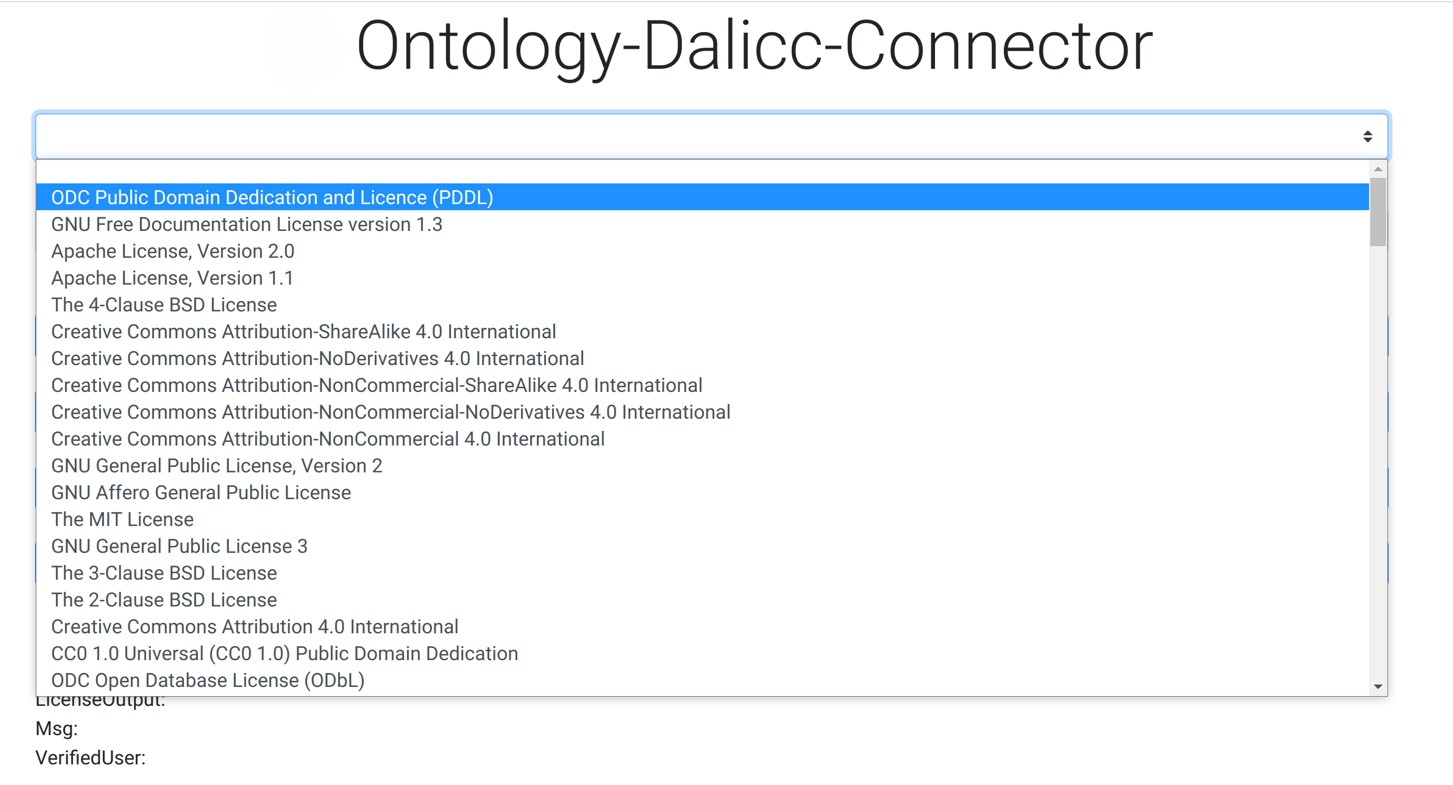
\includegraphics[width=1.95\textwidth]{images/chap03_selectType.jpg}
		\end{minipage}
		\caption[Define Type from DALICC library]{Define Type from DALICC library}
		
	\end{figure}
	
\end{center}
	\item Define Content:
	In this step, the user should choose the file or data that wants to be licensed. Subsequently, the hash \texttt{SHA3-256} of the selected file is calculated which is used to retrieve license information later.
 \begin{center}
	\begin{figure}[htb!]
		
		\begin{minipage}{0.45\linewidth}
			\centering
			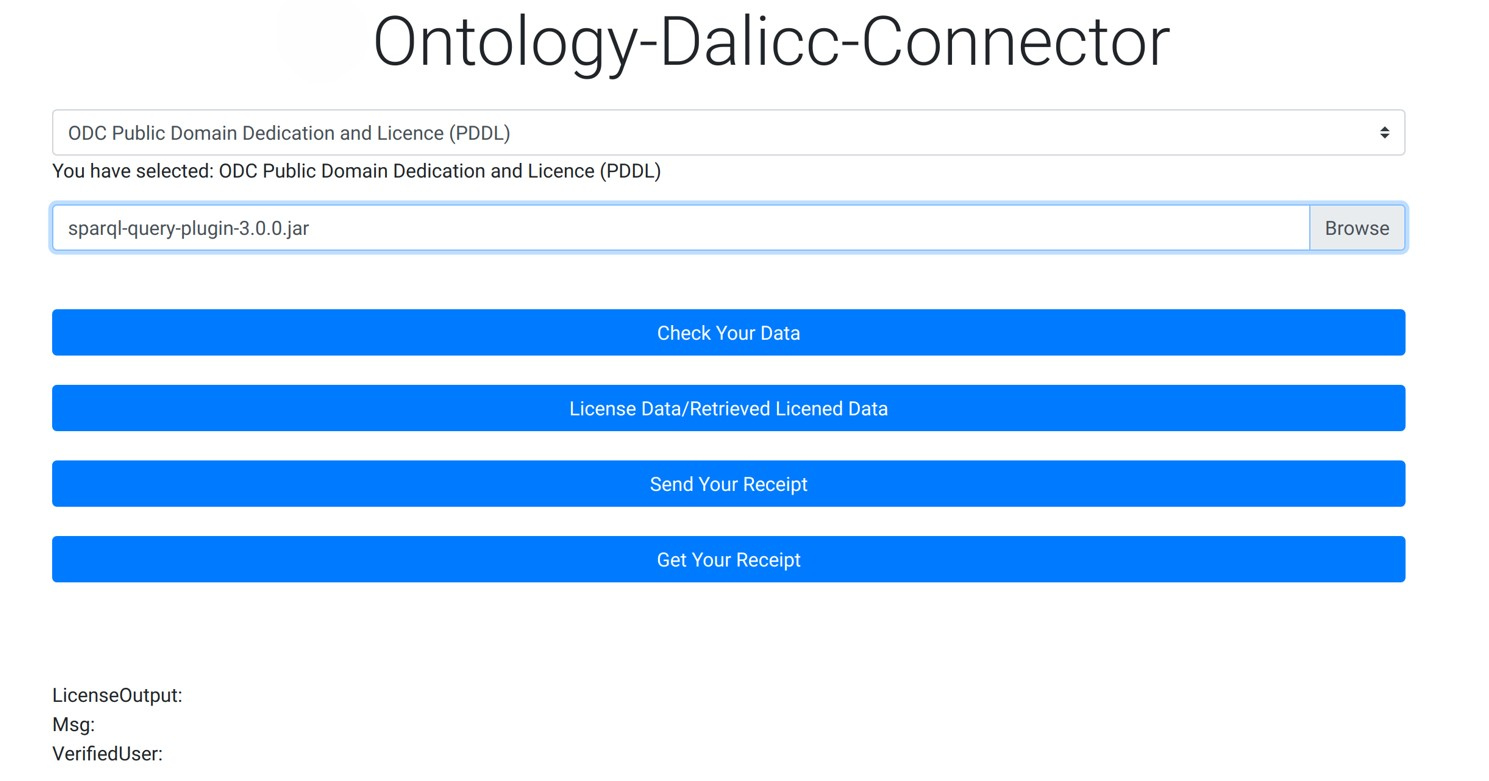
\includegraphics[width=1.95\textwidth]{images/chap03_selectFile.jpg}
		\end{minipage}
		\caption[Define file from local device]{Define file from local device}
		
	\end{figure}
\end{center}
	\item Check Your Data:
	In this step, the user should check the selected data: if it is licensed before or not. He/ she receives just a message either confirmation 'License is detected' or rejection 'License is not detected'. He or she should go further to obtain more information.
    \begin{center}
	\begin{figure}[htb!]
		
		\begin{minipage}{0.45\linewidth}
			\centering
			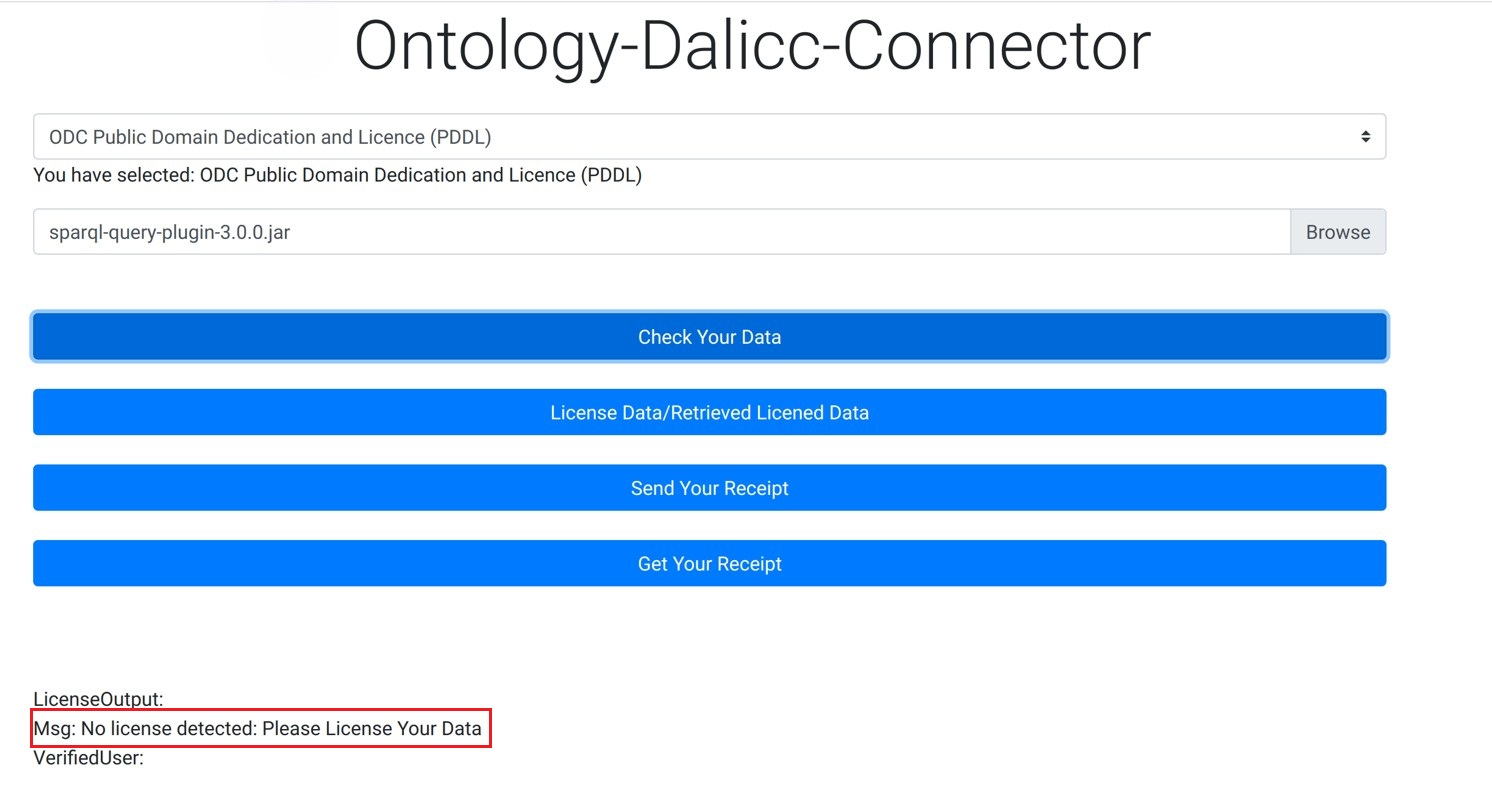
\includegraphics[width=1.95\textwidth]{images/chap03_checkFile.jpg}
		\end{minipage}
		\caption[Check if file is already licensed?]{Check if file is already licensed?}
		
	\end{figure}
	
\end{center}

\begin{center}
	\begin{figure}[htb!]
		
		\begin{minipage}{0.45\linewidth}
			\centering
			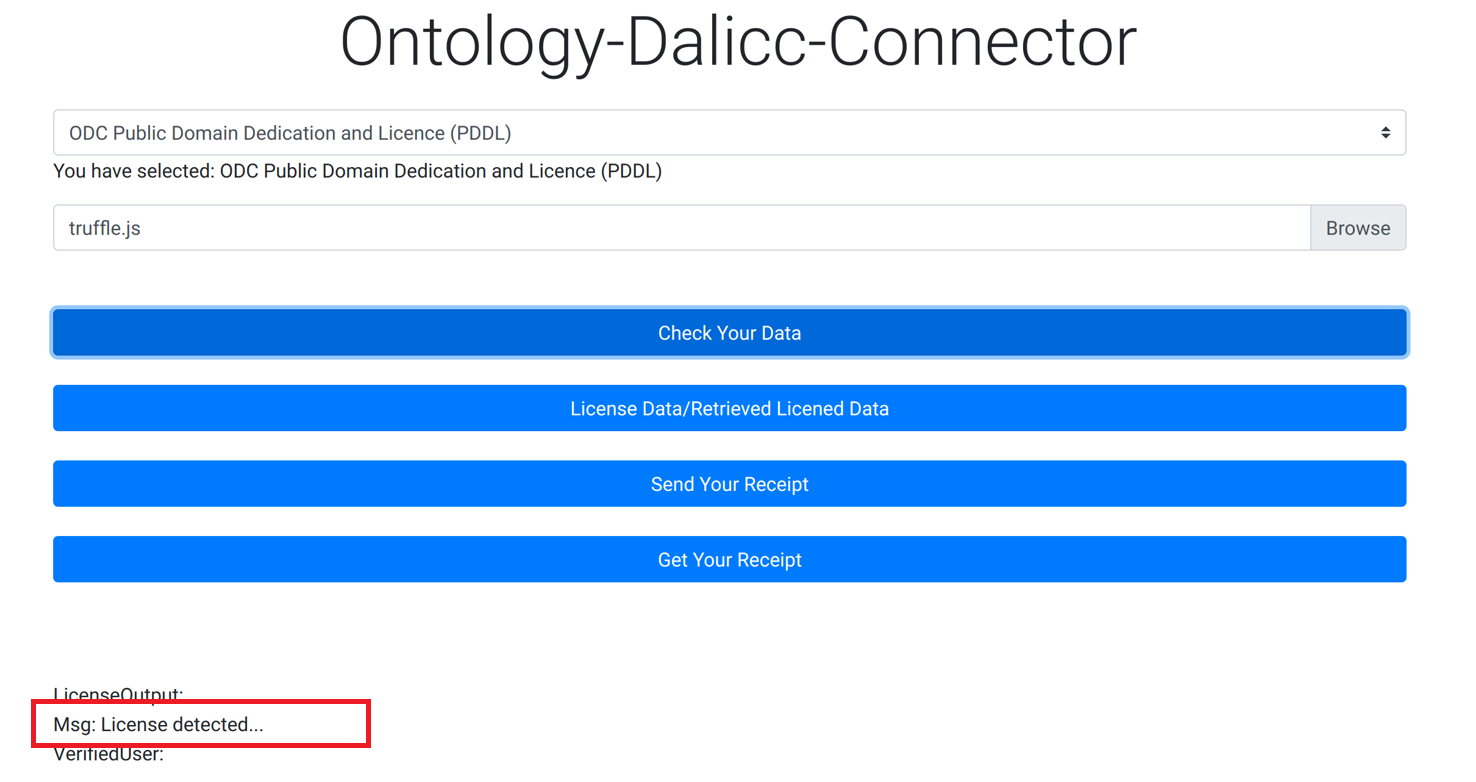
\includegraphics[width=1.95\textwidth]{images/chap03_found_license.png}
		\end{minipage}
		\caption[message for licensed data]{message for licensed data}
		
	\end{figure}
	
\end{center}
	\item License data / retrieve License information:
	Here, the user receives the result of that last step, by pressing the hash value of selected data \texttt{SHA3-256} is calculated and passed to the smart contract using \textit{web. js} interface: \\
    \\
	\textbf{- } License information of the selected file or data from which the user received the 'license detected' message from the last step. The user receives some information related to the license, licensor address, and URI related to the license.\\
    \begin{center}
	\begin{figure}[htb!]
		
		\begin{minipage}{0.55\linewidth}
			\centering
			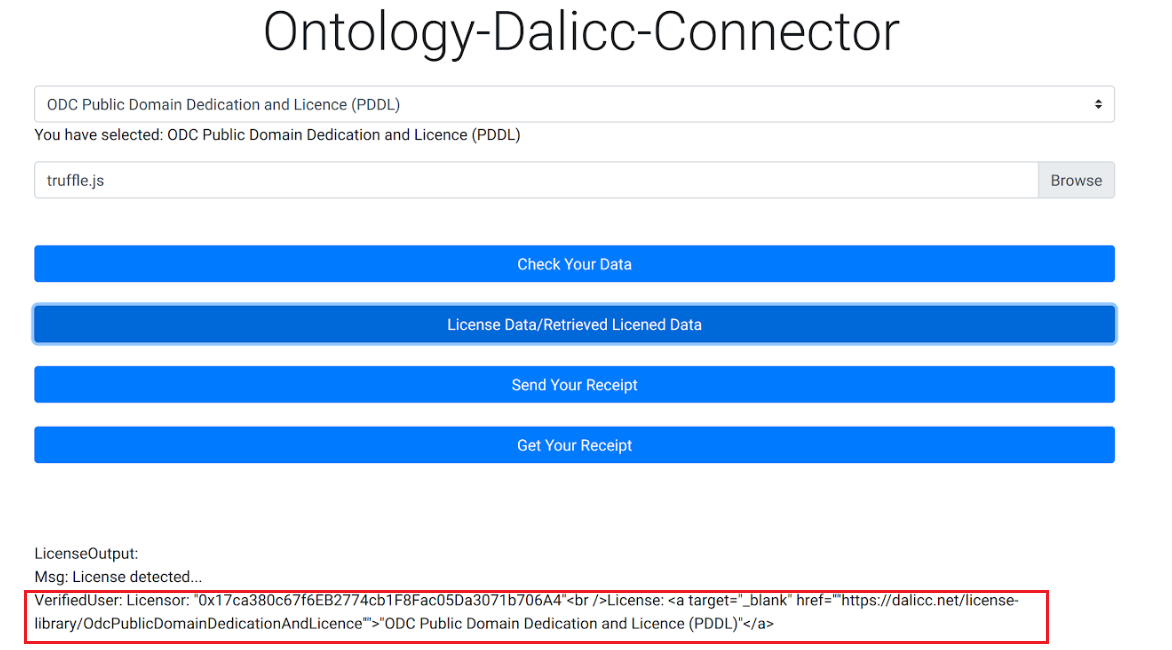
\includegraphics[width=1.95\textwidth]{images/chap03_found_info.png}
		\end{minipage}
		\caption[license information for already licensed data]{license information for already licensed data}
		
	\end{figure}
	
\end{center}
    \textbf{- } Start licensing he/her file, if he/she received 'No license detected'  from the last step. To license data, the user gets asked to log into \texttt{Metamask} to pass this account as the address of the licensor to the smart contract. The SHA3-256 hash value is calculated and passed by the contract to the Web3 Javascript interface. Users can see this hash in the front end, depending on the successful transaction or he/she receives the error message for failed transaction on the front end.\\
    \begin{center}
	 \begin{figure}[htb!]
		\begin{minipage}{0.45\linewidth}
			\centering
			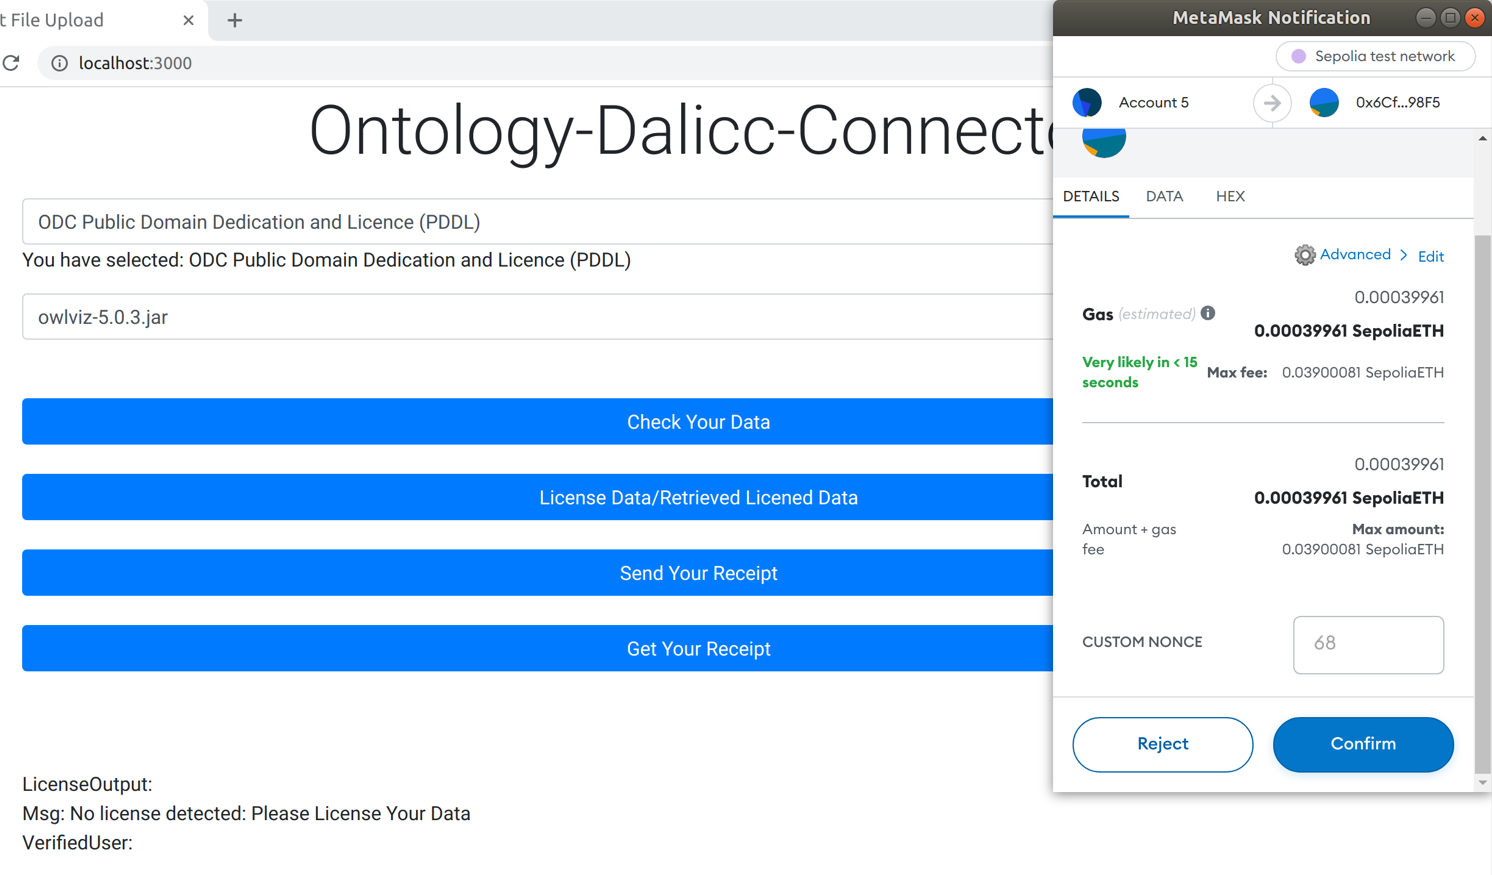
\includegraphics[width=1.95\textwidth]{images/chap03_license_data.png}
		\end{minipage}
		\caption[licensing data process]{licensing data process}
		
	\end{figure}
\end{center}
   \begin{center}
	\begin{figure}[htb!]
		
		\begin{minipage}{0.45\linewidth}
			\centering
			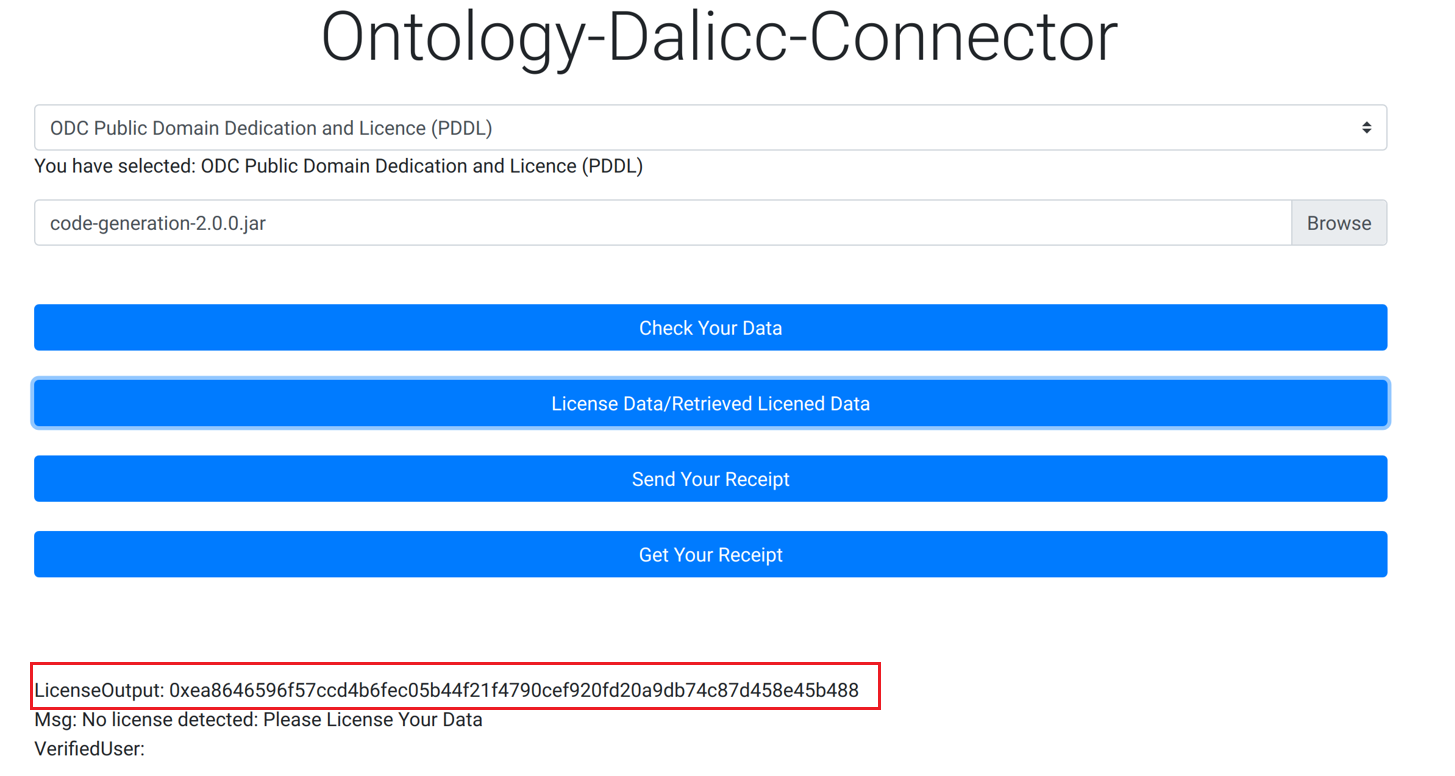
\includegraphics[width=1.95\textwidth]{images/chap03_license_hash.png}
		\end{minipage}
		\caption[License hash after confirming transaction]{License hash after confirming transaction}
		
	\end{figure}
\end{center}
   

\begin{center}
	\begin{figure}[htb!]
		
		\begin{minipage}{0.45\linewidth}
			\centering
			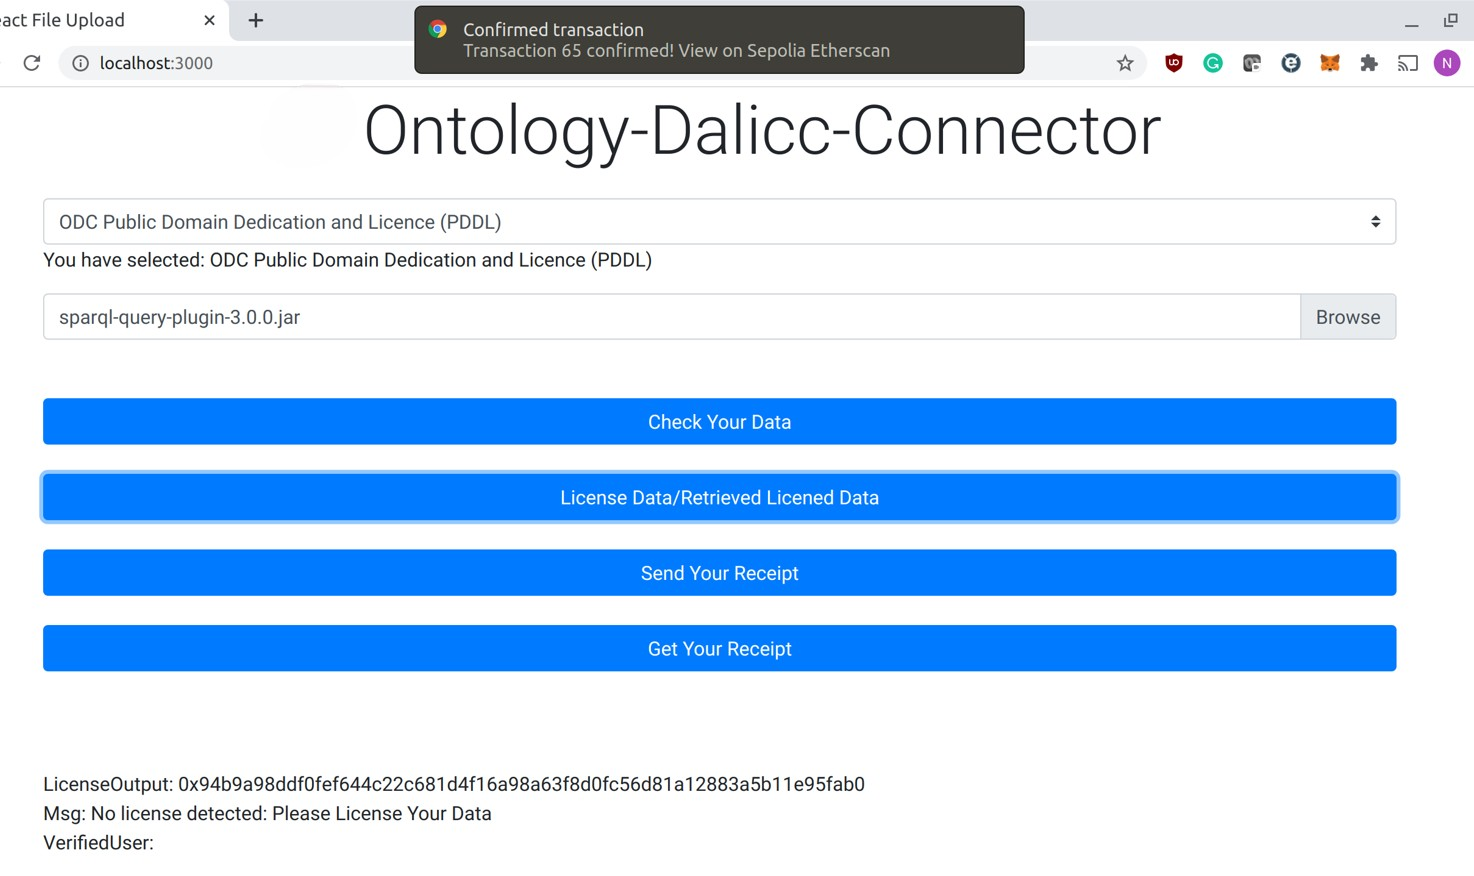
\includegraphics[width=1.95\textwidth]{images/chap03_confirm_tx.jpg}
		\end{minipage}
		\caption[Transaction confirmation]{Transaction confirmation}
		
	\end{figure}
	
\end{center}
	\item Send transaction: After receiving the hash of the transaction in the frontend, the user goes further to get a receipt of this licensing having all details about the transaction. to have this receipt user sends a transaction receipt that is not readable to the server for more processing on this raw result, converting to RDF format data and making a query to produce more readable RDF-based data.
	\item Get Transaction receipt:
	In the last step, the user can get a receipt of all transactions that have been done till now as a table in RDF format.
\end{itemize}

\begin{center}
	\begin{figure}[htb!]
		
		\begin{minipage}{0.55\linewidth}
			\centering
			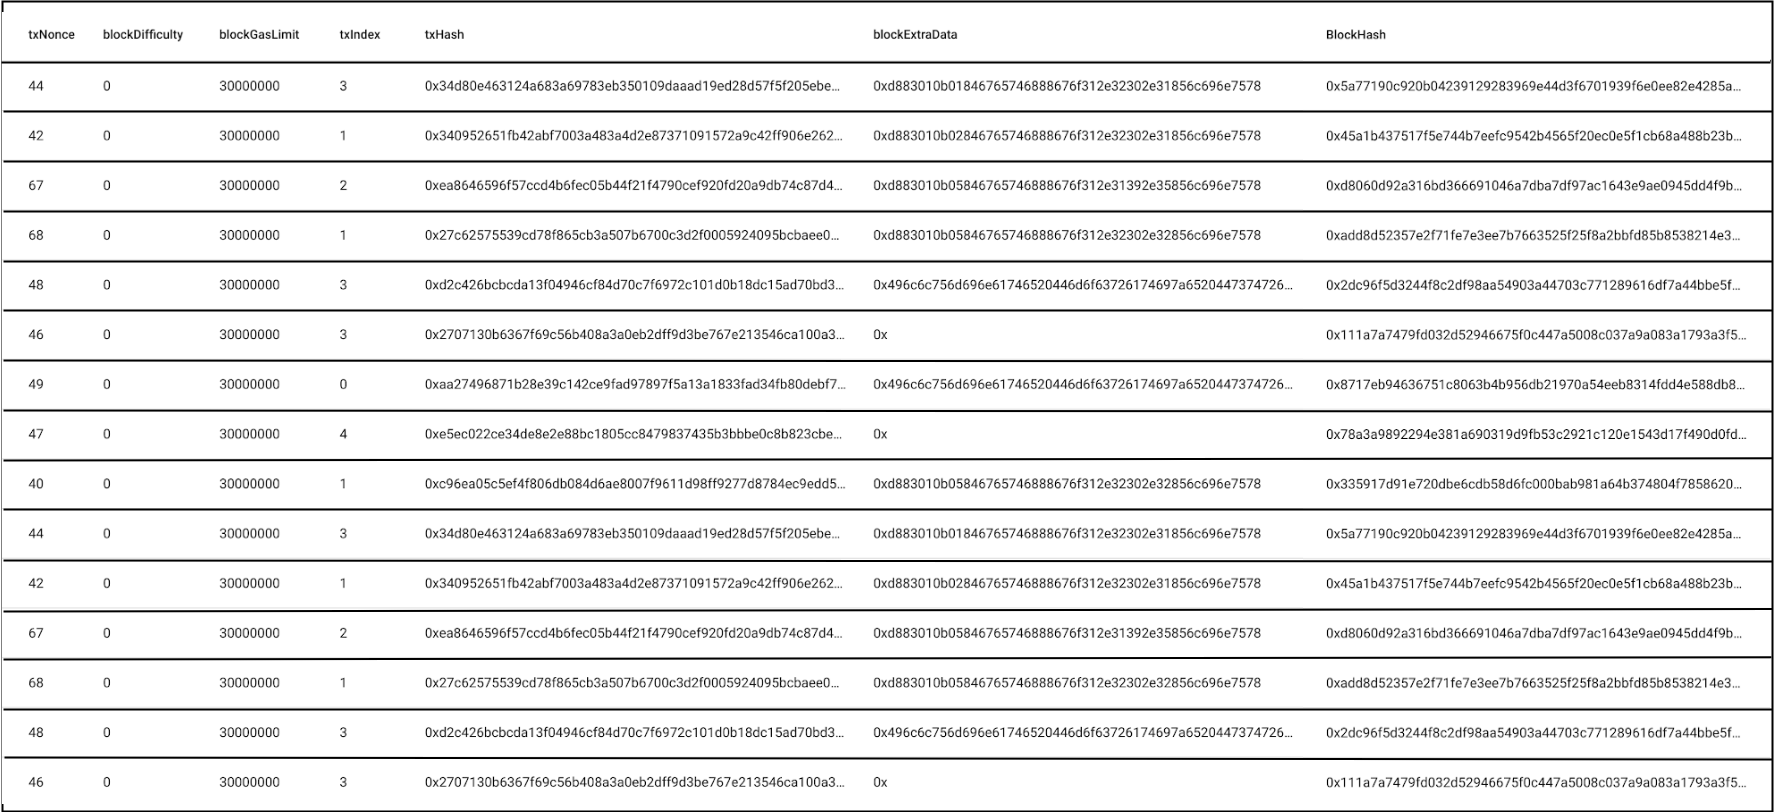
\includegraphics[width=1.95\textwidth]{images/chap03_licese_result_1.png}
		\end{minipage}
		\caption[Result of semantic mapping]{Result of semantic mapping}
		
	\end{figure}
	
\end{center}
\begin{center}
	\begin{figure}[htb!]
		
		\begin{minipage}{0.55\linewidth}
			\centering
			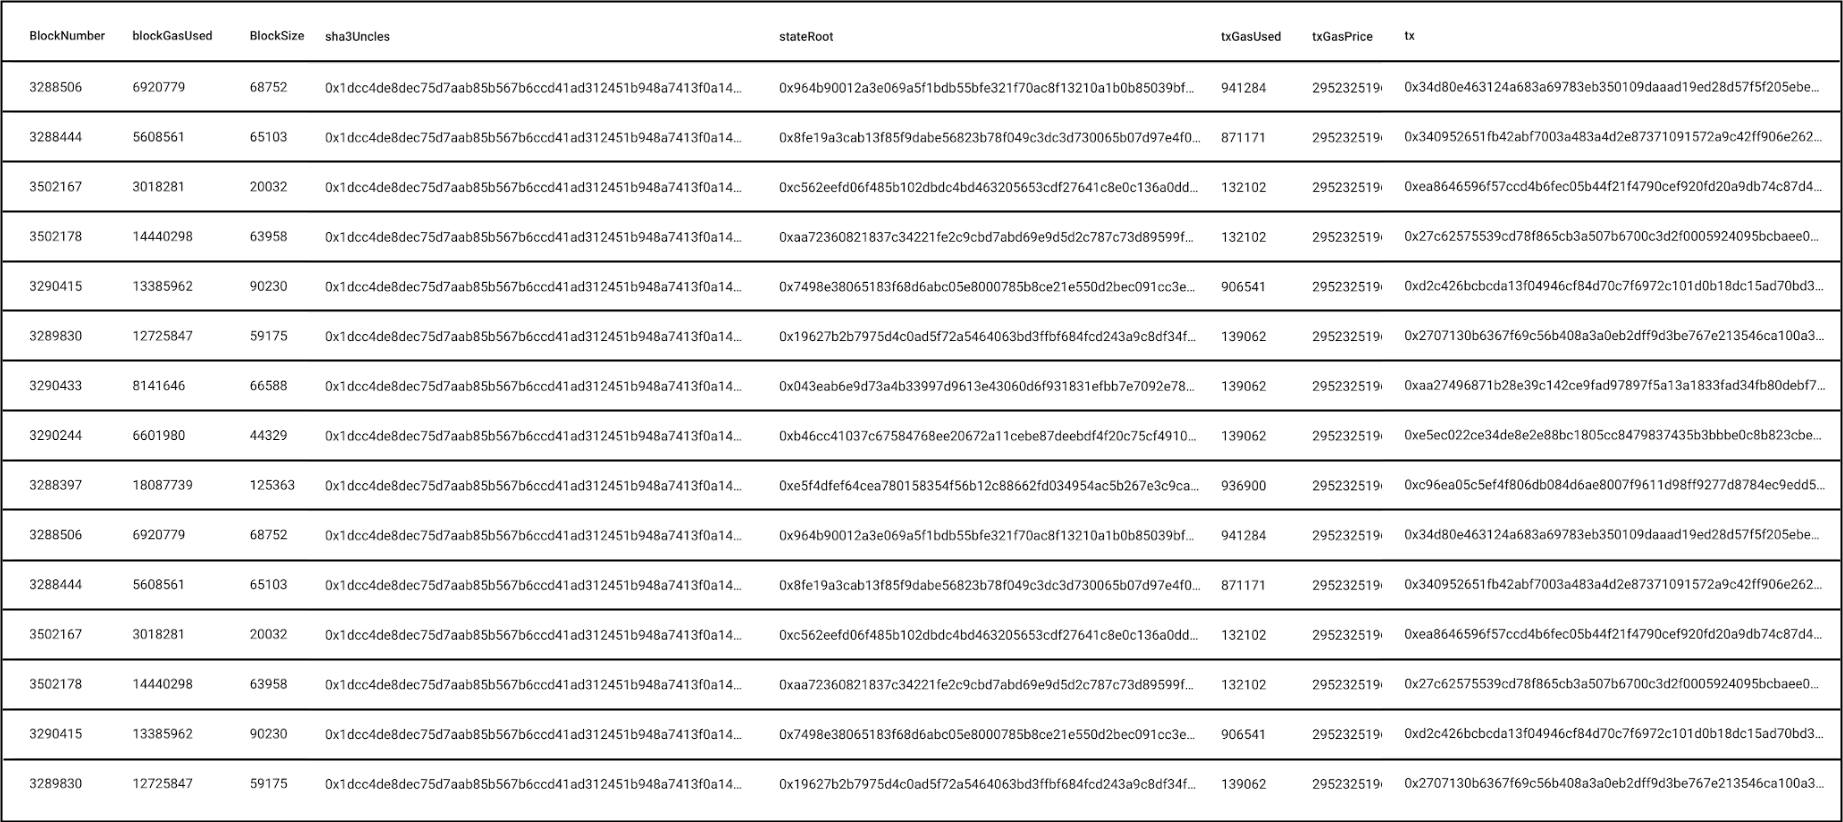
\includegraphics[width=1.95\textwidth]{images/chap03_licese_result_2.png}
		\end{minipage}
		\caption[Result of semantic mapping]{Result of semantic mapping}
		
	\end{figure}
	
\end{center}